\chapter{Testing e Performance}
\section{Testing}
    Per i test dell'applicazione sono stati utilizzati:
    \begin{itemize}
        \item \href{https://www.scalatest.org/}{Scala Test} versione 3.2.14 per il \textit{model} dell'applicazione
        \item \href{https://junit.org/junit5/}{JUnit 5} e \href{https://github.com/TestFX/TestFX}{TestFx} versione 4.0.16-alpha per l'interfaccia grafica
    \end{itemize}
    
    Come già detto nel capitolo \ref{chap:impl} relativo all'implementazione, si è prestata particolare attenzione nell'eseguire test dettagliati sui componenti del \textit{model}, assicurando quindi che gli elementi del dominio rappresentati all'interno del programma fossero sufficientemente robusti.
    Nella figura \ref{fig:coverage} è possibile osservare la coverage del \textit{model}, realizzata attraverso il tool \href{https://github.com/scoverage/sbt-scoverage}{Scoverage}, consultabile anche nella \href{https://isiquiz.github.io/PPS-22-isiquiz/coverage/}{documentazione online} del progetto.
    Per quanto riguarda la \textit{view}, sono stati realizzati test utilizzando TestFX per assicurarsi che le interfacce grafiche rispettassero i vincoli imposti dal domain expert.
    Per la \textit{view} non è disponibile la coverage relativa ai test a causa della difficile integrazione tra Scoverage e la suite di testing TestFX, tuttavia, l'applicazione è stata testata da almeno cinque persone esterne al team di sviluppo. Esse hanno utilizzato diverse versioni dei più diffusi e moderni sistemi operativi includendo Windows, Linux e MacOS e hanno sottolineato una buona qualità dell'interfaccia grafica soprattutto per quanto riguarda l'usabilità di essa.
    \begin{figure}[H]
        \centering
        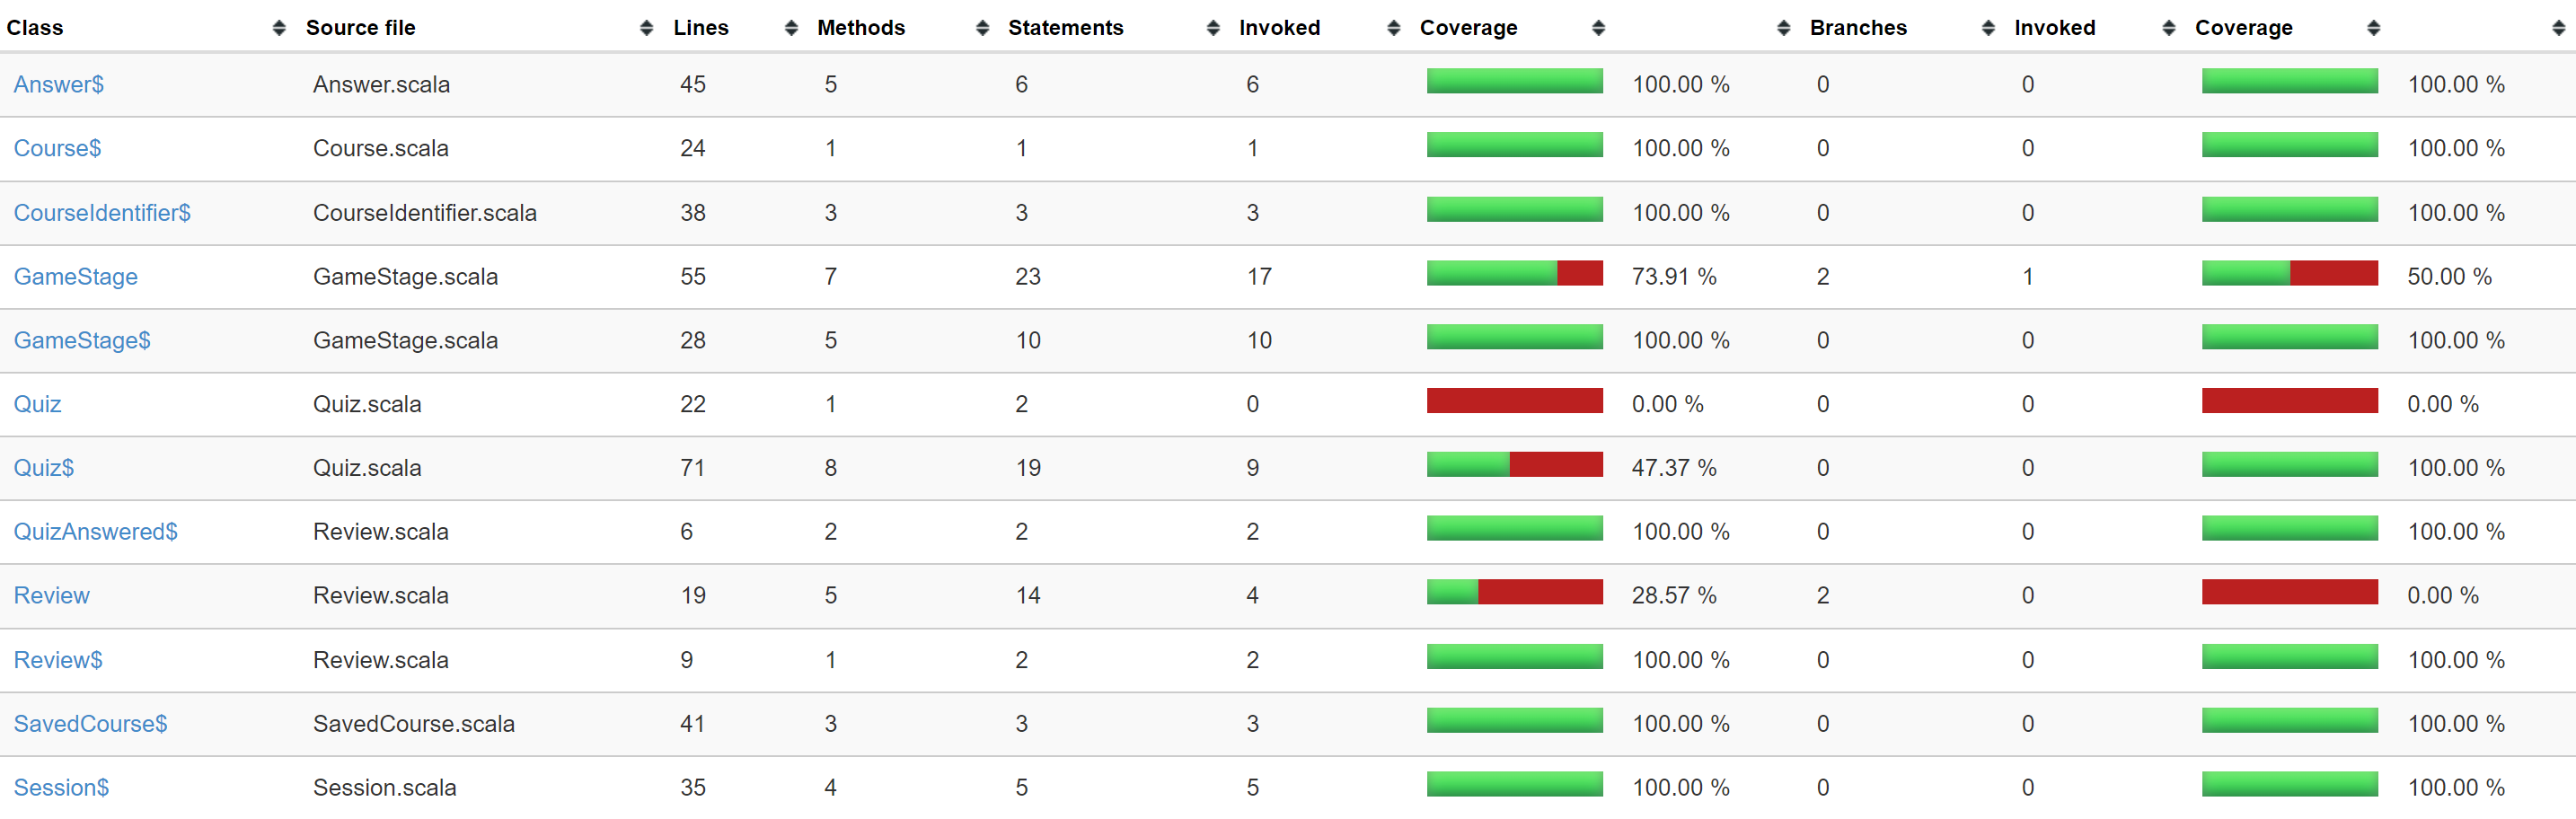
\includegraphics[width=\textwidth]{Images/coverage.png}
        \caption{Coverage del \textit{model}}
        \label{fig:coverage}
    \end{figure}

\section{Performance}
    Per quanto riguarda le performance, il programma è stato eseguito con successo su diversi dispositivi e sistemi operativi (nello specifico Windows, Linux e MacOS). Si riportano in Figura \ref{fig:visualvm} i risultati dell'esecuzione di una partita standard osservata attraverso il tool \href{https://visualvm.github.io/}{VisualVM}.
    \begin{figure}[H]
        \centering
        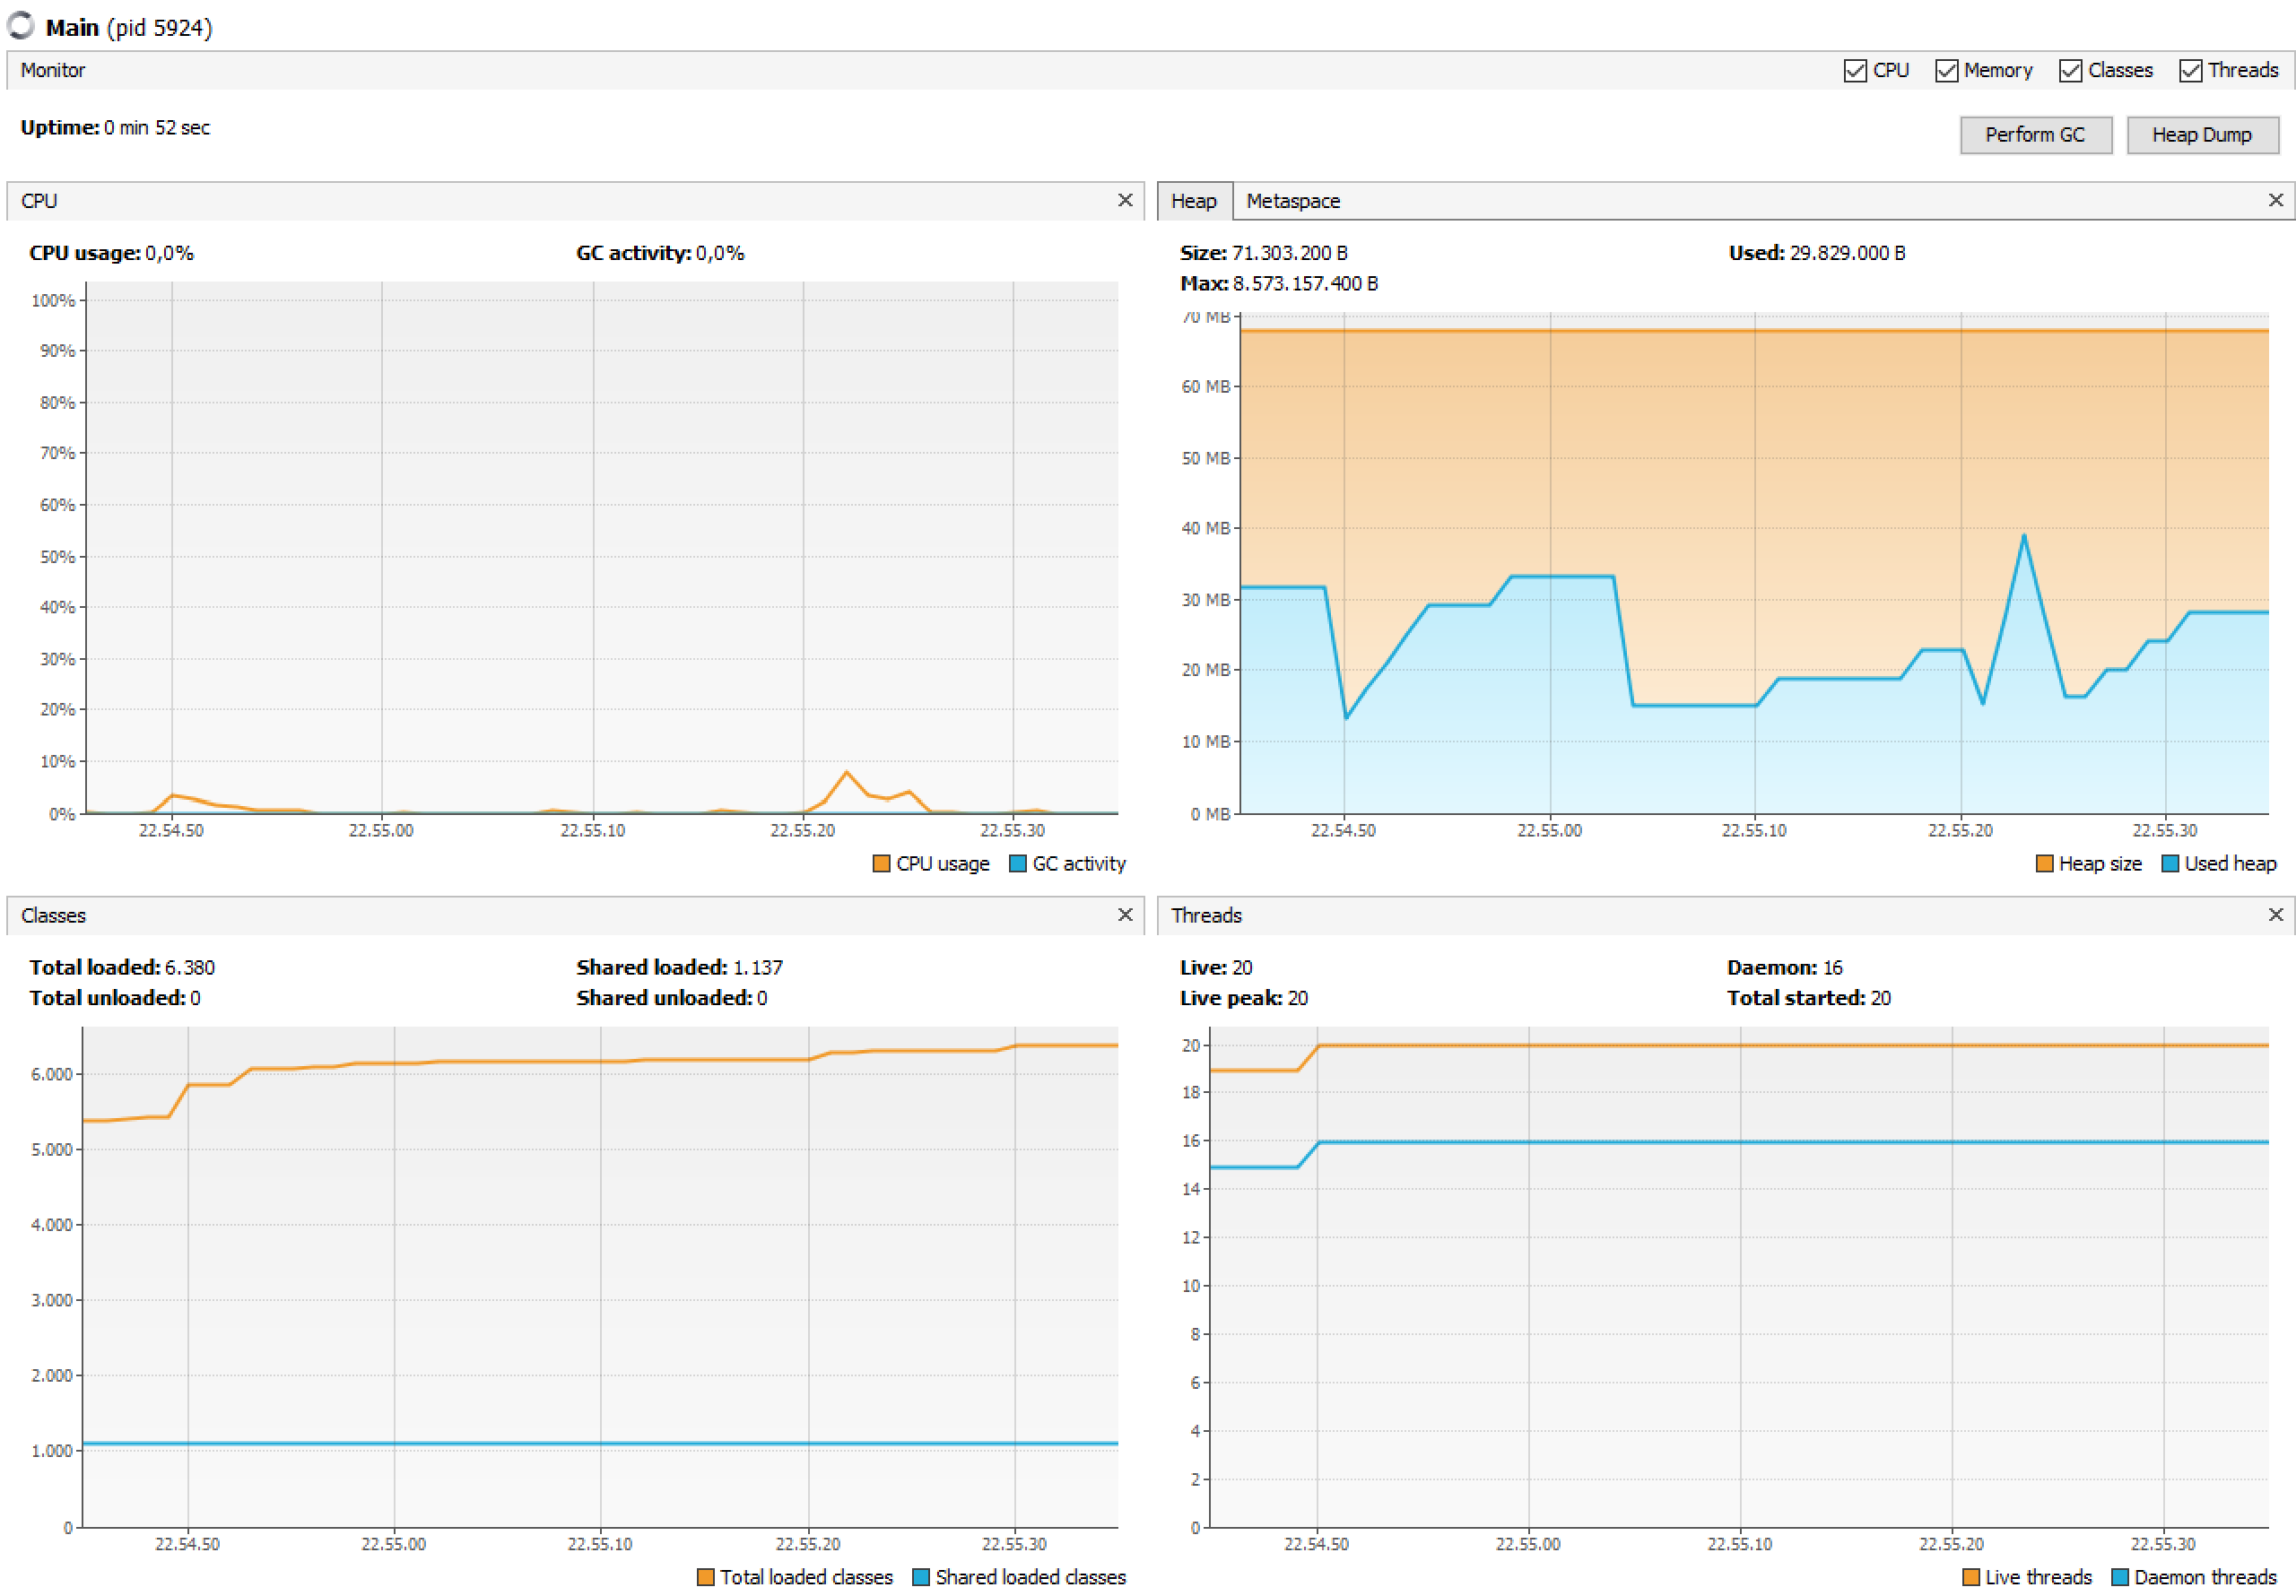
\includegraphics[width=\textwidth]{Images/VisualVM.png}
        \caption{Monitoraggio esecuzione di una partita}
        \label{fig:visualvm}
    \end{figure}